% Enable warnings about problematic code
\RequirePackage[l2tabu, orthodox]{nag}

\documentclass{WeSTassignment}

% The lecture title, e.g. "Web Information Retrieval".
\lecture{Introduction to Web Science}
% The names of the lecturer and the instructor(s)
\author{%
  Prof. Dr.~Steffen~Staab\\{\normalsize\mailto{staab@uni-koblenz.de}} \and
  Ren{\'e}~Pickhardt\\{\normalsize\mailto{rpickhardt@uni-koblenz.de}} \and
   Korok~Sengupta\\{\normalsize\mailto{koroksengupta@uni-koblenz.de}}
}
% Assignment number.
\assignmentnumber{5}
% Institute of lecture.
\institute{%
  Institute of Web Science and Technologies\\%
  Department of Computer Science\\%
  University of Koblenz-Landau%
}
% Date until students should submit their solutions.
\datesubmission{November 30, 2016, 10:00 a.m.}
% Date on which the assignments will be discussed in the tutorial.
\datetutorial{December 2, 2016, 12:00 p.m.}

% Set langauge of text.
\setdefaultlanguage[
  variant = american, % Use American instead of Britsh English.
]{english}

% Specify bib file location.
\addbibresource{bibliography.bib}

% For left aligned centerd boxes
% see http://tex.stackexchange.com/a/25591/75225
\usepackage{varwidth}

% ==============================================================================
% Document

\begin{document}

\maketitle
Please look at the lessons 1) \textbf{Dynamic Web Content} \& 2) \textbf{How big is the Web?}

For all the assignment questions that require you to write code, make sure to include the code in the answer sheet, along with a separate python file. Where screen shots are required, please add them in the answers directly and not as separate files.\\ \\ 

%Please mention your team Names here: 
Team Name: papa
\\Members: Brigitte Aznar
\\Bonasmitha Behura
\\Ilia Tugushi

% ------------------------------------------------------------------------------
\section{Creative use of the Hyptertext Transfer Protocol (10 Points)}
HTTP is a request response protocol. In that spirit a client opens a TCP socket to the server, makes a request, and the server replies with a response. The server will just listen on its open socket but cannot initiate a conversation with the client on its own. 

However you might have seen some interactive websites which notify you as soon as something happens on the server. An example would be Twitter. Without the need for you to refresh the page (and thus triggering a new HTTP request) they let you know that there are new tweets available for you. In this exercise we want you to make sense of that behaviour and try to reproduce it by creative use of the HTTP protocol.

Have a look at \texttt{server.py}\footnote{you could store the code from \url{http://blog.wachowicz.eu/?p=256} in a file called \texttt{server.py}} and \texttt{webclient.html} (which we provide). Extend both files in a way that after \texttt{webclient.html} is servered to the user the person controlling the server has the chance to make some input at its commandline. This input should then be send to the client and displayed automatically in the browser without requiring a reload. For that the user should not have to interact with the webpage any further.

\subsection{webclient.html}
\begin{lstlisting}
<html>
<head>
	<title>Abusing the HTTP protocol - Example</title>
</head>
<body>
	<h1>Display data from the Server</h1>
	The following line changes on the servers command line
	input: <br>
	<span id="response" style="color:red">
		This will be replaced by messages from the server
	</span>
</body>
</html>
\end{lstlisting}

\subsection{Hints:}
\begin{itemize}
\item This exercise is more like a riddle. Try to focuse on how TCP sockets and HTTP work and how you could make use of that to achieve the expected behaviour. Once you have an idea the programming should be straight-forward. 
\item The Javascript code that you need for this exercise was almost completely shown in one of the videos and is available on Wikiversity.
\item In that sense we only ask for a "proof of concept" nothing that would be stable out in the wilde.
  \begin{itemize}
  	\item In particular, don't worry about making the server uses multithreading. It is ok to be blocking for the sake of this exercise.
  \end{itemize}
\item Without use of any additional libraries or AJAX framework we have been able to solve this with 19 lines of Javascript and 11 lines of Python code (we provide this information just as a way for you to estimate the complexity of the problem, don't worry about how many lines your solution uses).
\end{itemize}

\textbf{\\Answer:}
For the sake of saving paper, we are only pasting here the relevant part of the code for the exercise.\\
\begin{lstlisting}
 while True:
         print ("Awaiting New connection")
         self.socket.listen(3) # maximum number of queued connections
         
         conn, addr = self.socket.accept()
         # conn - socket to client
         # addr - clients address
         
         data = conn.recv(1024) #receive data from client
         string = bytes.decode(data) #decode it to string

         # split on space "GET /file.html" -into-> ('GET','file.html',...)
         file_requested = string.split(' ')
         file_requested = file_requested[1]  # get 2nd element

         # Check for URL arguments. Disregard them
         file_requested = file_requested.split('?')[0]  # disregard anything after '?'

         if (file_requested == '/'):  # in case no file is specified by the browser
             file_requested = '/index.html'  # load index.html by default

         file_requested = self.www_dir + file_requested
         file_requested = file_requested.strip("/")
         print("Serving web page [", file_requested, "]")

         ## Load file content
         try:
             file_handler = open(file_requested,'rb')
             if (request_method == 'GET'):  #only read the file when GET
                 response_content = file_handler.read() # read file content
             file_handler.close()

             response_headers = self._gen_headers( 200)

         except Exception as e: #in case file was not found, generate 404 page
             if file_requested == "server":
                 inpt = input("Say somethin nice to the user: ")
                 conn.send(self._gen_headers( 200).encode() + inpt.encode())
                 conn.close()
                 continue
             else:
                 print ("Warning, file not found. Serving response code 404\n", e)
                 response_headers = self._gen_headers( 404)

                 #if (request_method == 'GET'):
                 response_content = b"<html><body><p>Error 404: File not found</p><p>Python HTTP server</p></body></html>"


         server_response =  response_headers.encode() # return headers for GET and HEAD
         #if (request_method == 'GET'):
         server_response +=  response_content   # return additional conten for GET only

         conn.send(server_response)
         print ("Closing connection with client")
         conn.close()
\end{lstlisting}


% ------------------------------------------------------------------------------
\section{Web Crawler (10 Points)}
Your task in this exercise is to "crawl" the \texttt{Simple English Wikipedia}. In order to execute this task, we provide you with a mirror of the Simple English Wikipedia at \url{141.26.208.82}. 

You can start crawling from \url{http://141.26.208.82/articles/g/e/r/Germany.html} and you can use the \texttt{urllib} or \texttt{doGetRequest} function from the last week's assignment.

Given below is the strategy that you might adopt to complete this assignment: 
\begin{enumerate}
\item Download \url{http://141.26.208.82/articles/g/e/r/Germany.html} and store the page on your file system. 
\item Open the file in python and extract the local links. (Links within the same domain.)
\item Store the file to your file system.
\item Follow all the links and repeat steps 1 to 3.
\item Repeat step 4 until you have downloaded and saved all pages. 
\end{enumerate}

\subsection{Hints:}
\begin{itemize}
\item Before you start this exercise, please have a look at Exercise 3. 
\item Make really sure your crawler doesn't follow external urls to domains other than \mbox{\url{http://141.26.208.82}}. In that case you would start crawling the entire web
\item Expect the crawler to run about 60 Minutes if you start it from the university network. From home your runtime will most certainly be even longer.
\item It might be useful for you to have some output on the crawlers commandline depicting which URL is currently being fetched and how many URLs have been fetched so far and how many are currently on the queue.
\item You can (but don't have to) make use of breadth-first search.
\item It probably makes sense to take over the full paths from the pages of the Simple English Wikipedia and use the same folder structure when you save the html documents.
\item You can (but you don't have to) speed up the crawler significantly if you use multithreading. However you should not use more than 10 threads in order for our mirror of Simple English Wikipedia to stay alive. 
\end{itemize}

% ------------------------------------------------------------------------------

\section{Web Crawl Statistics (10 Points)}

If you have successfully completed the first exercise of this assignment, then please provide the following details. You may have to tweak your code in the above exercise for some of the results. 
\subsection{Phase I}
\begin{enumerate}
\item Total Number of \emph{webpages} you found.
\item Total number of links that you encountered in the complete process of crawling.
\item Average and median number of links per web page.
\item Create a \emph{histogram} showing the distribution of links on the crawled web pages. You can use a bin size of 5 and scale the axis from 0-150.
\end{enumerate}

\subsection{Phase II}
\begin{enumerate}
\item For every page that you have downloaded, count the number of internal links and external links. 
\item Provide a \emph{scatter plot} with number of internal links on the X axis and number of external links on the Y axis.
\end{enumerate}

\textbf{Answer: }
\\Code for parts II and III
\begin{lstlisting}
import os
import re
import urllib
import numpy as npy
from collections import deque
import matplotlib.pyplot as plt
from urllib.parse import urljoin
import matplotlib.patches as mpatches

total_num_links = []
num_external_links = []
num_internal_links = []


# def get_links(file_name, qurl):
def get_links(data, qurl):
    links = []
    links_to_return = []
    internal = 0
    external = 0
    domain = 'http://141.26.208.82'

    # regex to check the a tag
    hrefs = re.compile(r'<\s*a [^>]*href="([^"]+)')

    # with open(file_name, encoding="utf8") as file:
    #     for line in file:
    #         reg = hrefs.findall(line)
    #         if reg:
    #             links.extend(reg)

    regex = hrefs.findall(data)
    if regex:
        links.extend(regex)

    for link in links:
        if link.find(domain) > -1 or link.find('http') != 0:
            internal += 1
            #Dont include links that starts with #
            if link.find('#') != 0:
                link = urljoin(qurl, link)
                links_to_return.append(link)
        else:
            external += 1

    num_external_links.append(external)
    num_internal_links.append(internal)
    total_num_links.append(internal + external)

    return links_to_return

def plot():
    plt.scatter(num_internal_links, num_external_links)

    # adds labels to the axis
    plt.xlabel('Internal Links')
    plt.ylabel('External Links')

    # generates legend
    legend = mpatches.Patch(color='blue', label='Number of link in page')
    plt.legend(handles=[legend])
    plt.title("Number of Internal and External links in pages")
    plt.show()
    return plt

def histogram(total_links):
    total_links = npy.transpose(total_links)
    plt.hist(total_links, bins=5, range =(0,150))
    plt.title("Histogram with 'auto' bins")
    return plt

def main():

    path_to_file = os.path.realpath('.') + '\\wikipedia_crawl'
    os.makedirs(path_to_file, exist_ok=True)
    url = 'http://141.26.208.82/articles/g/e/r/Germany.html'
    #url = 'http://localhost/wikipedia-simple-html/simple/articles/g/e/r/Germany.html'
    queue = deque([url])
    visited = set()
    web_page = set()

    while True:
        if queue:
            element = queue.popleft()
            file_name = element.split('/')[-1]
            if file_name.find(".html") == -1:
                visited.add(element)
                continue
            if element not in visited:
                try:
                    response = urllib.request.urlopen(element)
                    data = response.read()
                    response.close()
                    visited.add(element)
                    web_page.add(element)

                    with open(os.path.join(path_to_file, file_name), 'wb') as file_to_write:
                       file_to_write.write(data)
                       file_to_write.close()

                    if len(web_page) % 1000 == 0:
                        print("pages downloaded: ", len(web_page))
                    print(element)
                    queue.extend(get_links(data.decode(), element))
                except Exception:
                    visited.add(element)
                    #print("Couldn't download " + element)
                    pass
        else:
            break

    print("Hurray! you just crawled simple english wikipedia")

    total_web_pages  = len(web_page)
    total_visited   = sum(total_num_links)
    avg = total_visited / total_web_pages
    median = npy.median(total_num_links)

    print("Now some statistics:")
    print("Phase I")
    print("----------------------------------------")
    print("Total number of web pages visited: ", total_web_pages)
    print("Total number of links encountered: ", total_visited)
    print("Average number of links per website: ", avg)
    print("Median of links per website: ", median)
    hist = histogram(total_num_links)
    hist.show()
    scatter = plot()
    scatter.show()

if __name__ == "__main__":
            main()

\end{lstlisting}

\textbf{Outputs:}
\begin{figure}[h]
  \centering
  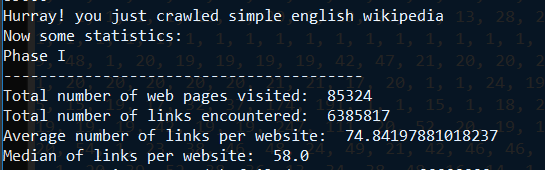
\includegraphics{statistics.png}
   \caption{Results of the statistics\\Being: Total number of websites visited: Total Websites downloaded}
     \label{fig:dig} 
\end{figure}


\begin{figure}[h]
  \centering
  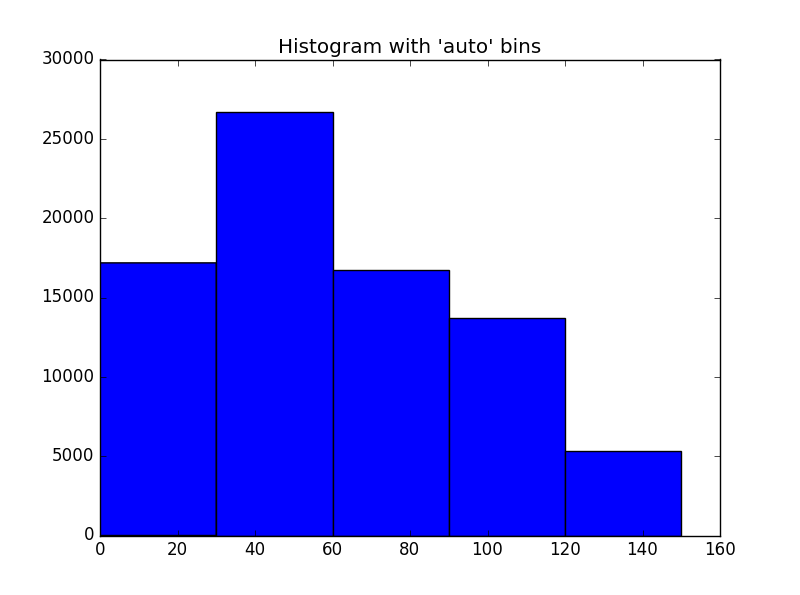
\includegraphics{histogram.png}
   \caption{X axis number of websites, Y axis links encountered}
     \label{fig:dig} 
\end{figure}


\begin{figure}[h]
  \centering
  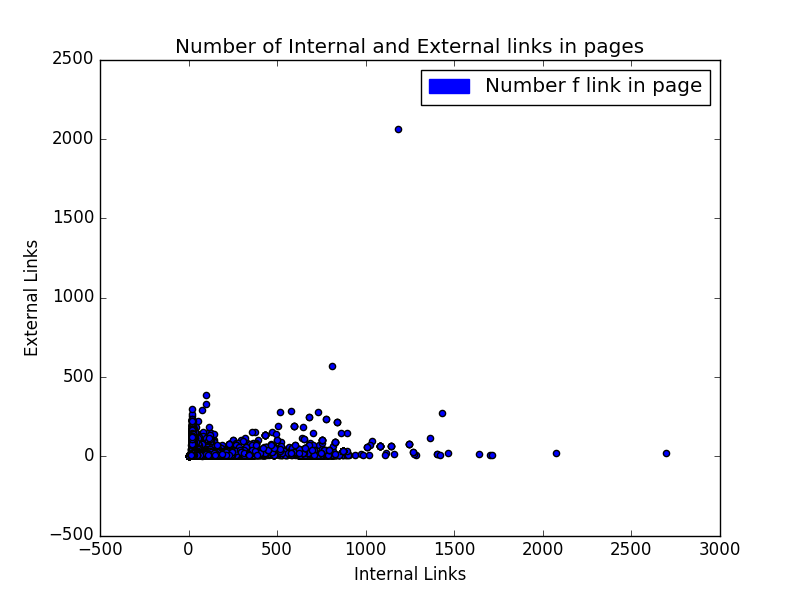
\includegraphics{scatter.png}
   \caption{Internal Vs external links in pages}
     \label{fig:dig} 
\end{figure}
% ------------------------------------------------------------------------------





\makefooter

\end{document}
